\section{Вариант 7}

\subsection{Компьютер 1}
Конфигурация:
\begin{verbatim}
ip link set enp0s8  down
ip link set enp0s9  down
ip link set enp0s10 down

sysctl -w net.ipv4.ip_forward=1
sysctl -w net.ipv4.conf.enp0s8.rp_filter=0
sysctl -w net.ipv4.conf.enp0s9.rp_filter=0
sysctl -w net.ipv4.conf.enp0s10.rp_filter=0

ip    a flush enp0s8
ip -6 a flush enp0s8
ip    a flush enp0s9
ip -6 a flush enp0s9
ip    a flush enp0s10
ip -6 a flush enp0s10
ip    r flush default
ip -6 r flush default

ip link set enp0s8 up
ip    a a        5.6.1.1/24  dev enp0s8
ip -6 a a ::ffff:5.6.1.1/120 dev enp0s8

ip link set enp0s9 up
ip    a a        5.6.2.1/24  dev enp0s8
ip -6 a a ::ffff:5.6.2.1/120 dev enp0s8

ip link set enp0s10 up
ip    a a        5.6.3.1/24  dev enp0s8
ip -6 a a ::ffff:5.6.3.1/120 dev enp0s8

iptables  -t mangle -F
ip6tables -t mangle -F

ip    r a default via 127.0.0.1
ip -6 r a default via ::1

iptables  -t mangle -I OUTPUT     -p icmp   \
    --icmp-type   echo-reply -j MARK --set-mark 1
iptables  -t mangle -I PREROUTING -p icmp   \
    --icmp-type   echo-reply -j MARK --set-mark 2
ip6tables -t mangle -I OUTPUT     -p icmpv6 \
    --icmpv6-type echo-reply -j MARK --set-mark 1
ip6tables -t mangle -I PREROUTING -p icmpv6 \
    --icmpv6-type echo-reply -j MARK --set-mark 2

ip    rule a from all fwmark 1 lookup icmp1
ip -6 rule a from all fwmark 1 lookup icmp1
ip    rule a from all fwmark 2 lookup icmp2
ip -6 rule a from all fwmark 2 lookup icmp2

ip    r a default via        5.6.2.2 dev enp0s9  table icmp1
ip -6 r a default via ::ffff:5.6.2.2 dev enp0s9  table icmp1
ip    r a default via        5.6.3.3 dev enp0s10 table icmp2
ip -6 r a default via ::ffff:5.6.3.3 dev enp0s10 table icmp2
\end{verbatim}

\subsection{Компьютер 2}
Конфигурация:
\begin{verbatim}
ip link set enp0s8  down
ip link set enp0s9  down
ip link set enp0s10 down

sysctl -w net.ipv4.ip_forward=1
sysctl -w net.ipv4.conf.enp0s8.rp_filter=0
sysctl -w net.ipv4.conf.enp0s9.rp_filter=0
sysctl -w net.ipv4.conf.enp0s10.rp_filter=0

ip    a flush enp0s8
ip -6 a flush enp0s8
ip    a flush enp0s9
ip -6 a flush enp0s9
ip    a flush enp0s10
ip -6 a flush enp0s10
ip    r flush default
ip -6 r flush default

ip link set enp0s8 up
ip    a a        5.6.1.2/24  dev enp0s8
ip -6 a a ::ffff:5.6.1.2/120 dev enp0s8

ip link set enp0s9 up
ip    a a        5.6.2.2/24  dev enp0s8
ip -6 a a ::ffff:5.6.2.2/120 dev enp0s8

ip link set enp0s10 up
ip    a a        5.6.4.2/24  dev enp0s8
ip -6 a a ::ffff:5.6.4.2/120 dev enp0s8

iptables  -t mangle -F
ip6tables -t mangle -F

ip    r a default via 127.0.0.1
ip -6 r a default via ::1

iptables  -t mangle -I PREROUTING -p icmp   \
    --icmp-type   echo-reply -j MARK --set-mark 1
iptables  -t mangle -I OUTPUT     -p icmp   \
    --icmp-type   echo-reply -j MARK --set-mark 2
ip6tables -t mangle -I PREROUTING -p icmpv6 \
    --icmpv6-type echo-reply -j MARK --set-mark 1
ip6tables -t mangle -I OUTPUT     -p icmpv6 \
    --icmpv6-type echo-reply -j MARK --set-mark 2

ip    rule a from all fwmark 1 lookup icmp1
ip -6 rule a from all fwmark 1 lookup icmp1
ip    rule a from all fwmark 2 lookup icmp2
ip -6 rule a from all fwmark 2 lookup icmp2

ip    r a default via        5.6.2.1 dev enp0s9  table icmp2
ip -6 r a default via ::ffff:5.6.2.1 dev enp0s9  table icmp2
ip    r a default via        5.6.4.3 dev enp0s10 table icmp1
ip -6 r a default via ::ffff:5.6.4.3 dev enp0s10 table icmp1
\end{verbatim}

\subsection{Компьютер 3}
Конфигурация:
\begin{verbatim}
ip link set enp0s8 down
ip link set enp0s9 down

sysctl -w net.ipv4.ip_forward=1
sysctl -w net.ipv4.conf.enp0s8.rp_filter=0
sysctl -w net.ipv4.conf.enp0s9.rp_filter=0

ip    a flush enp0s8
ip -6 a flush enp0s8
ip    a flush enp0s9
ip -6 a flush enp0s9
ip    r flush default
ip -6 r flush default

ip link set enp0s8 up
ip    a a        5.6.3.3/24  dev enp0s8
ip -6 a a ::ffff:5.6.3.3/120 dev enp0s8

ip link set enp0s9 up
ip    a a        5.6.4.3/24  dev enp0s9
ip -6 a a ::ffff:5.6.4.3/120 dev enp0s9

iptables  -t mangle -F
ip6tables -t mangle -F

ip    r a default via 127.0.0.1
ip -6 r a default via ::1

iptables  -t mangle -I OUTPUT -p icmp   --icmp-type   \
    echo-request -d        5.6.1.1 -j MARK --set-mark 1
iptables  -t mangle -I OUTPUT -p icmp   --icmp-type   \
    echo-request -d        5.6.1.2 -j MARK --set-mark 2
ip6tables -t mangle -I OUTPUT -p icmpv6 --icmpv6-type \
    echo-request -d ::ffff:5.6.1.1 -j MARK --set-mark 1
ip6tables -t mangle -I OUTPUT -p icmpv6 --icmpv6-type \
    echo-request -d ::ffff:5.6.1.2 -j MARK --set-mark 2

ip    rule a from all fwmark 1 lookup icmp1
ip -6 rule a from all fwmark 1 lookup icmp1
ip    rule a from all fwmark 2 lookup icmp2
ip -6 rule a from all fwmark 2 lookup icmp2

ip    r a default via        5.6.4.2 dev enp0s9 table icmp1
ip -6 r a default via ::ffff:5.6.4.2 dev enp0s9 table icmp1
ip    r a default via        5.6.3.1 dev enp0s8 table icmp2
ip -6 r a default via ::ffff:5.6.3.1 dev enp0s8 table icmp2
\end{verbatim}

\subsection{Скриншоты выполнения}
\subsubsection{Хост 1}
\paragraph{IPv4}
\begin{center}
    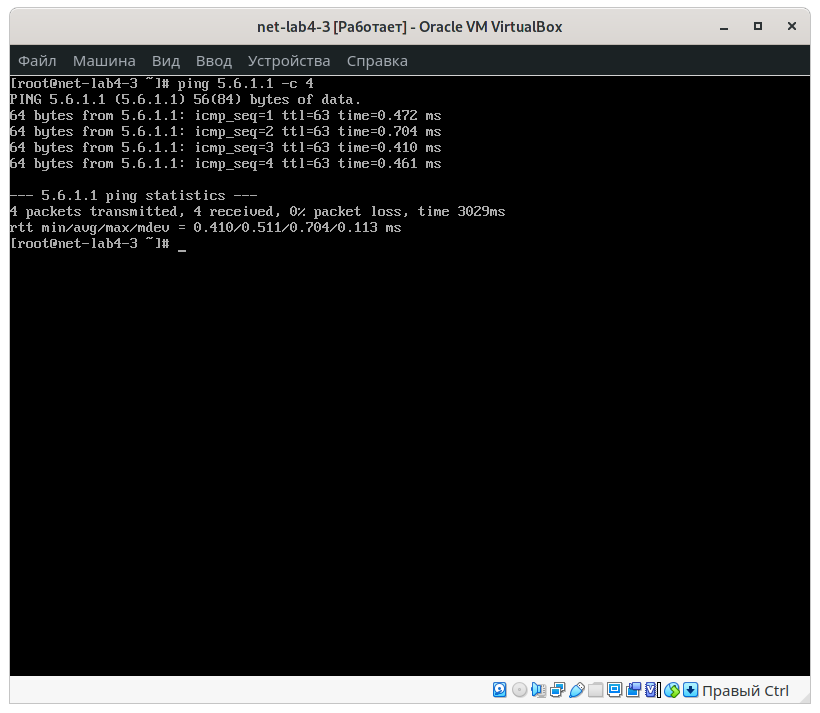
\includegraphics[width=.49\textwidth]{screenshots/var7-ping1-ipv4}
    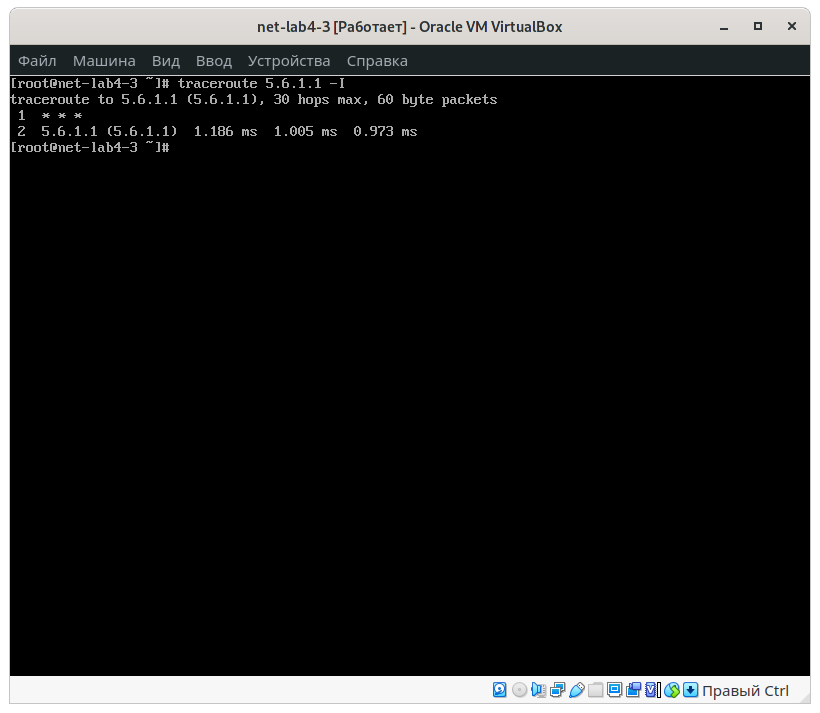
\includegraphics[width=.49\textwidth]{screenshots/var7-traceroute1-ipv4}

    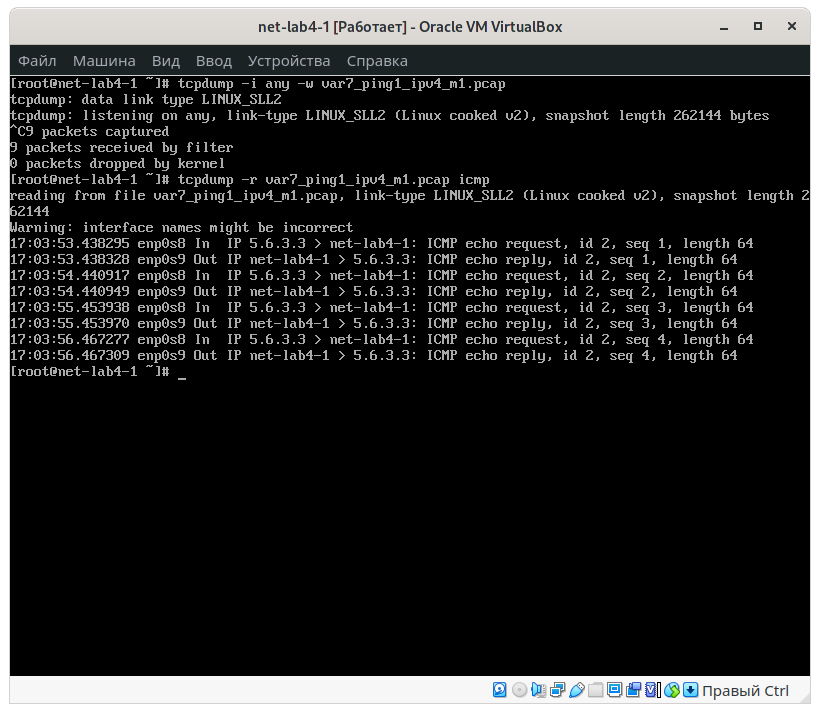
\includegraphics[width=.49\textwidth]{screenshots/var7-ping1-ipv4-tcpdump1}
    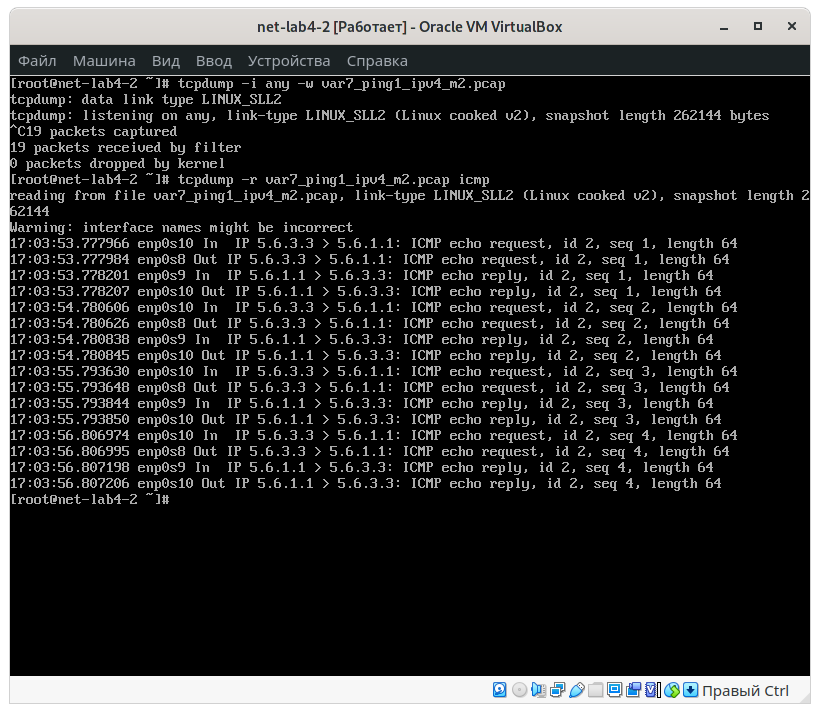
\includegraphics[width=.49\textwidth]{screenshots/var7-ping1-ipv4-tcpdump2}

%    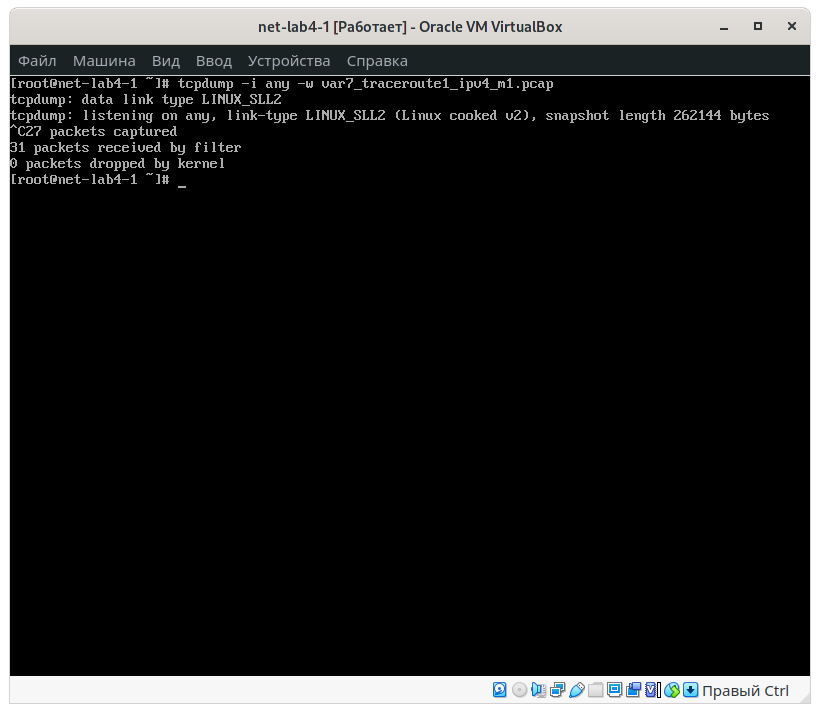
\includegraphics[width=.49\textwidth]{screenshots/var7-traceroute1-ipv4-tcpdump1}
%    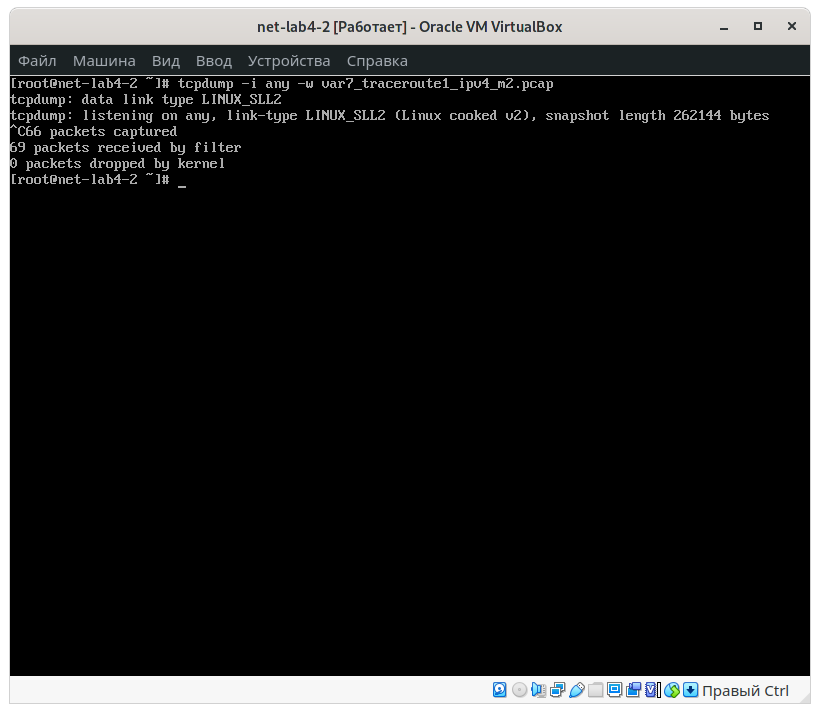
\includegraphics[width=.49\textwidth]{screenshots/var7-traceroute1-ipv4-tcpdump2}
\end{center}

\paragraph{IPv6}
\begin{center}
    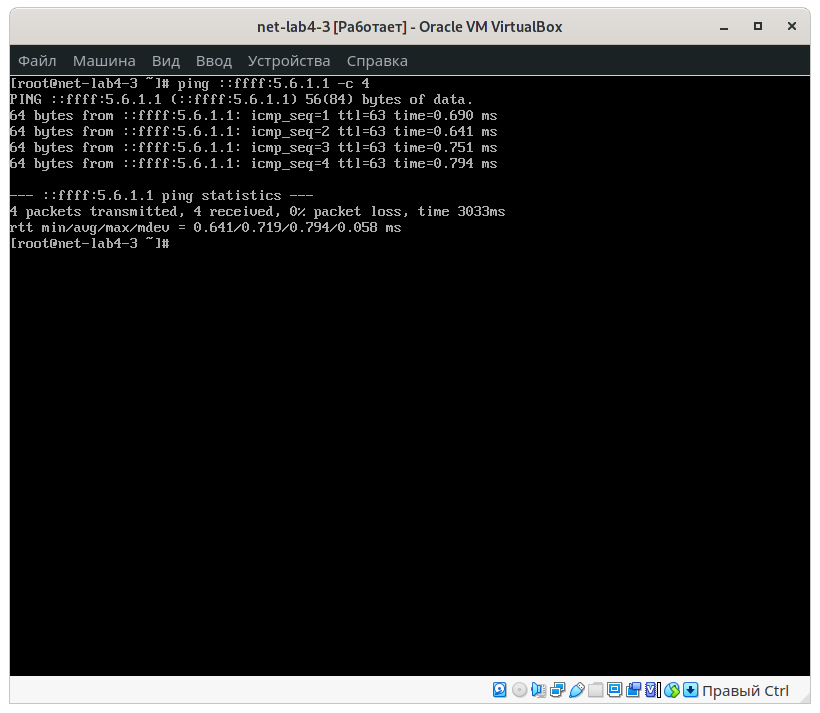
\includegraphics[width=.49\textwidth]{screenshots/var7-ping1-ipv6}
    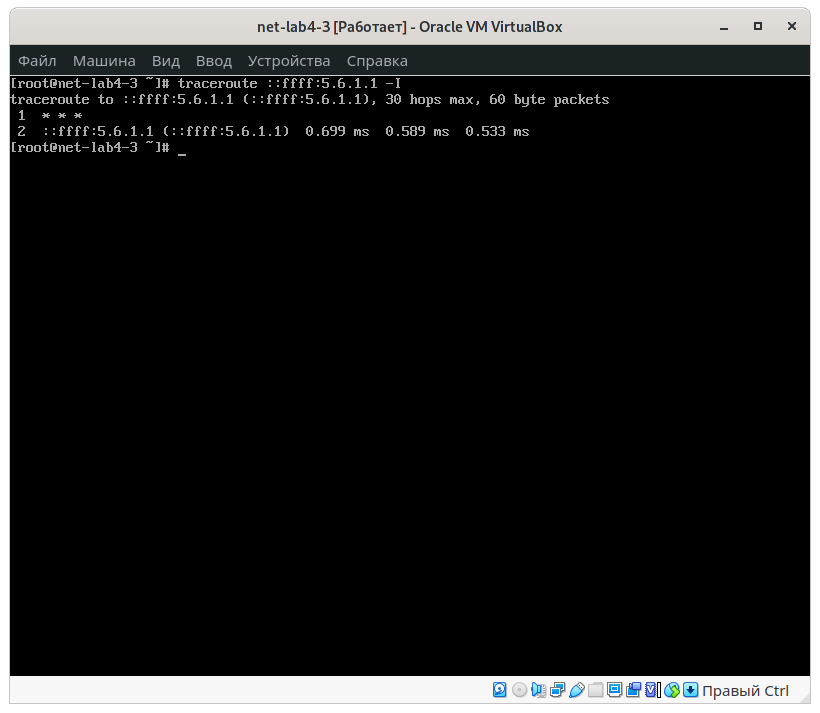
\includegraphics[width=.49\textwidth]{screenshots/var7-traceroute1-ipv6}

    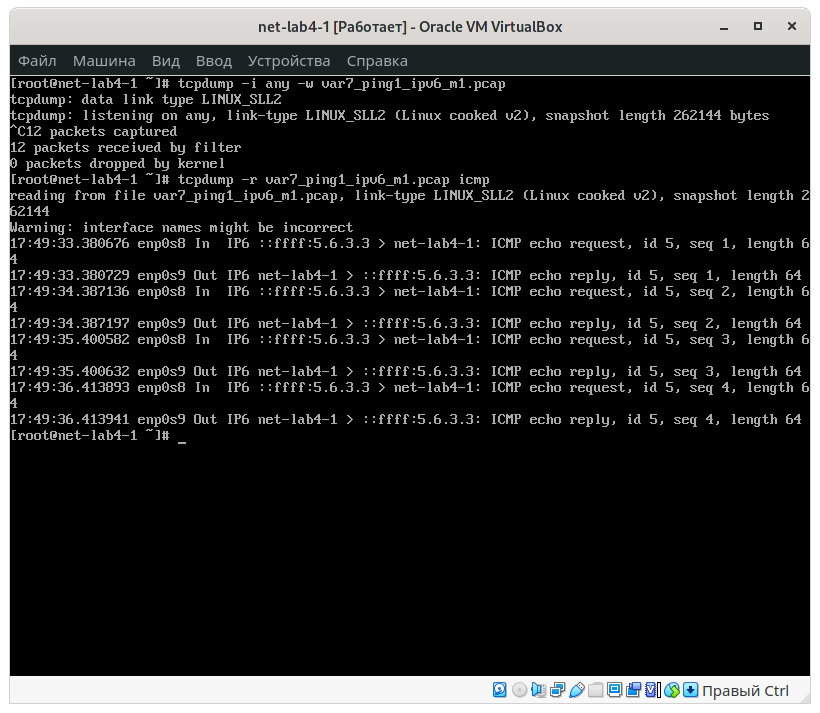
\includegraphics[width=.49\textwidth]{screenshots/var7-ping1-ipv6-tcpdump1}
    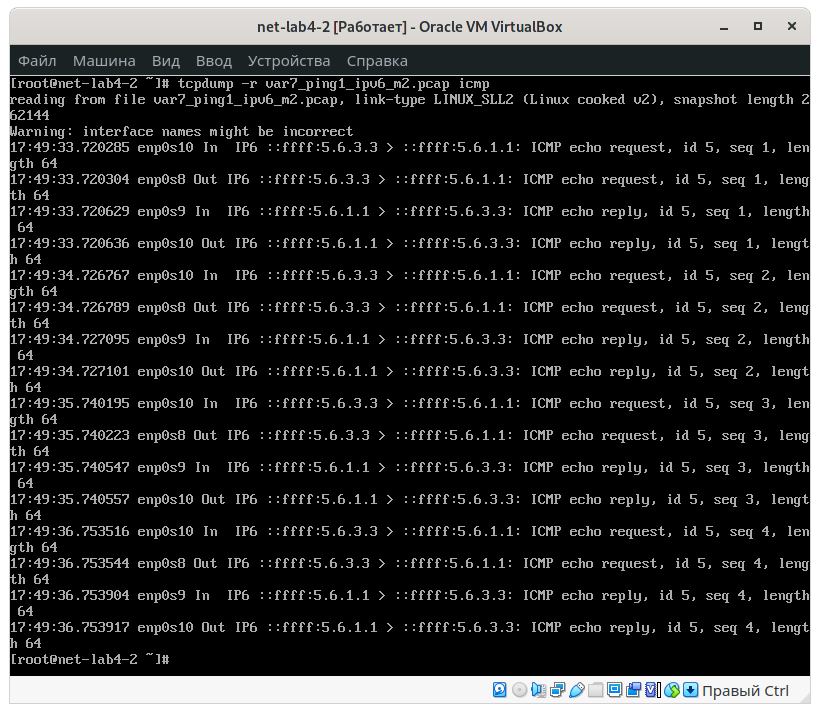
\includegraphics[width=.49\textwidth]{screenshots/var7-ping1-ipv6-tcpdump2}

%    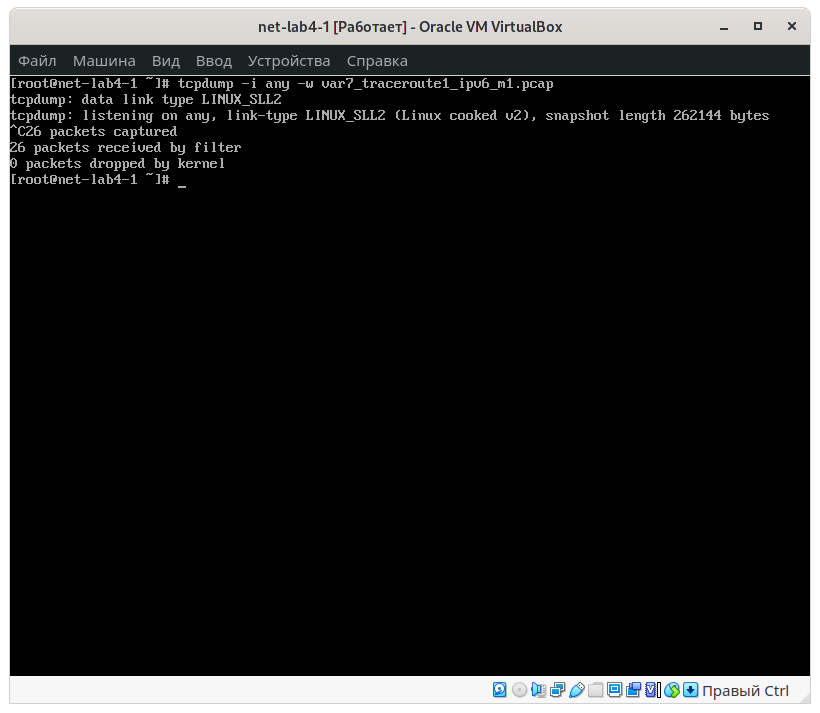
\includegraphics[width=.49\textwidth]{screenshots/var7-traceroute1-ipv6-tcpdump1}
%    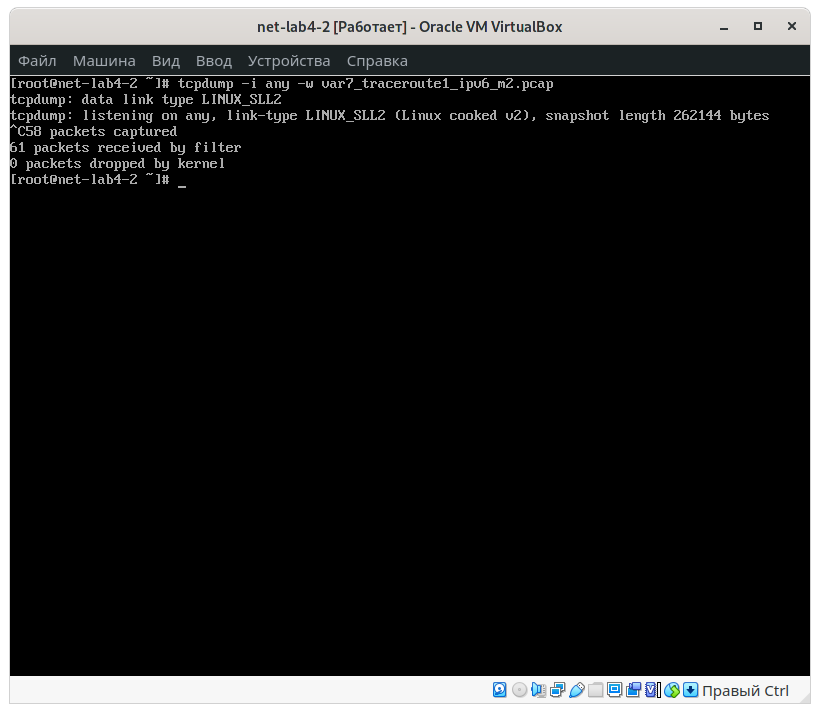
\includegraphics[width=.49\textwidth]{screenshots/var7-traceroute1-ipv6-tcpdump2}
\end{center}

\subsubsection{Хост 2}
\paragraph{IPv4}
\begin{center}
    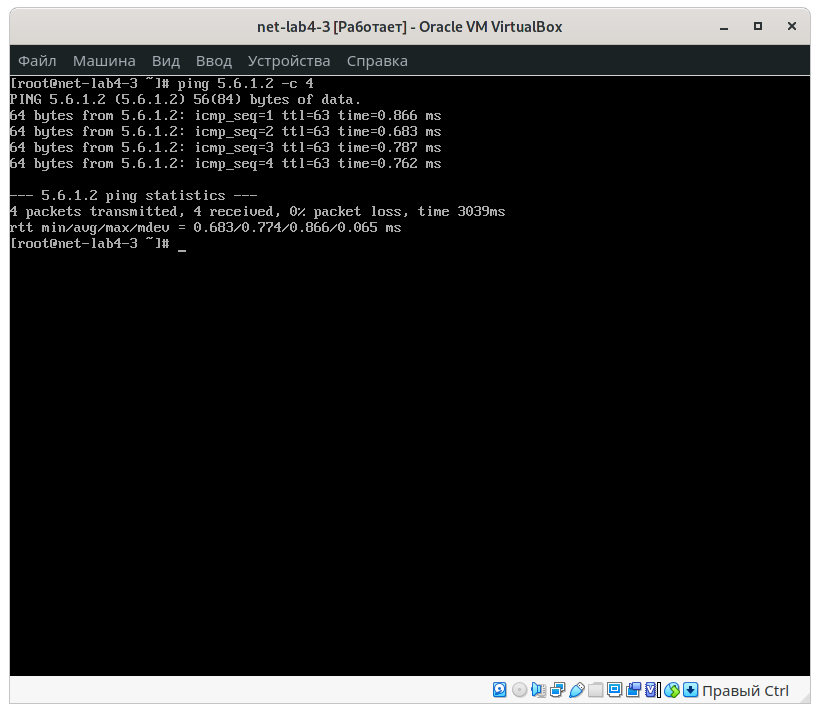
\includegraphics[width=.49\textwidth]{screenshots/var7-ping2-ipv4}
    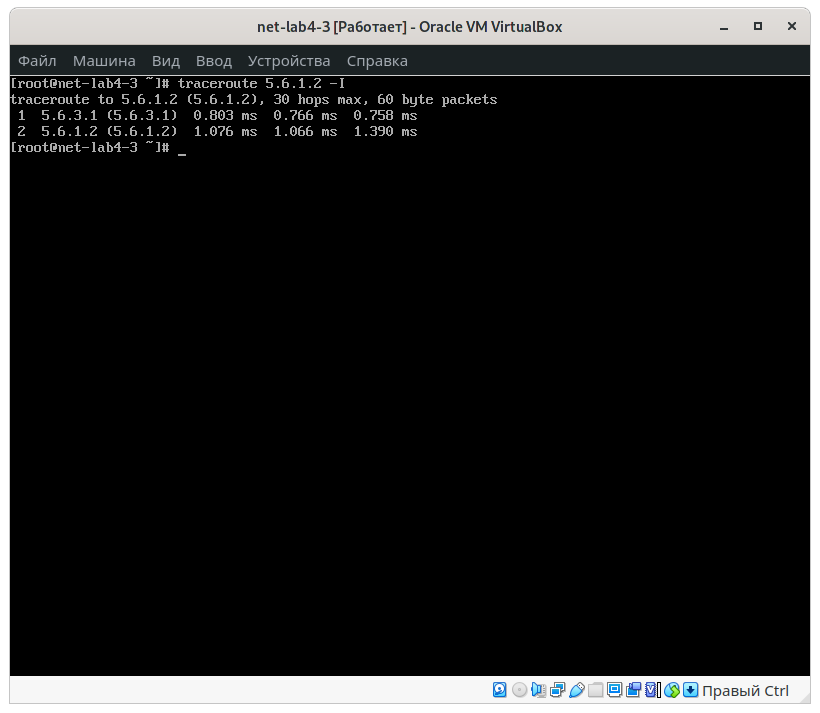
\includegraphics[width=.49\textwidth]{screenshots/var7-traceroute2-ipv4}

    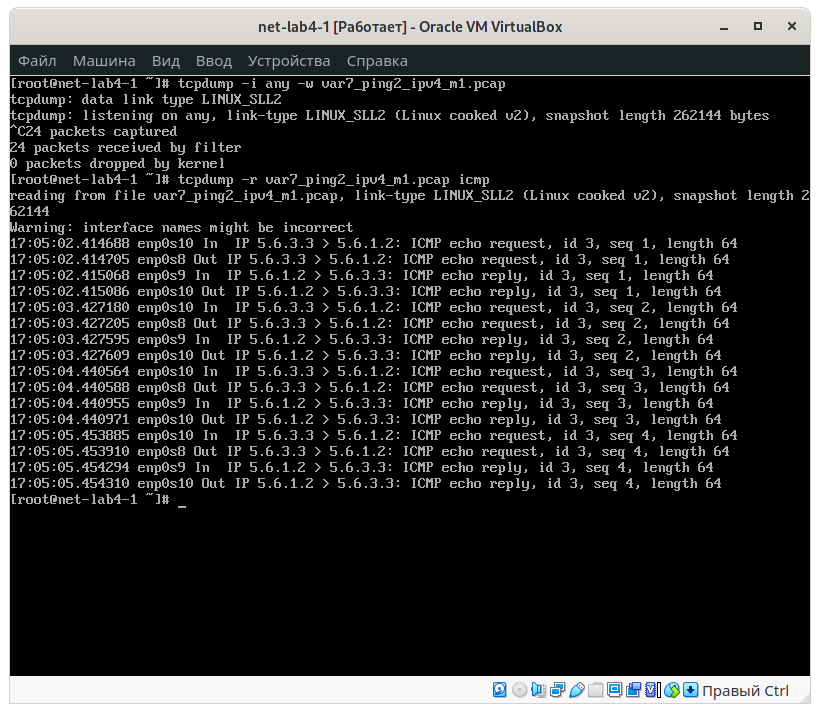
\includegraphics[width=.49\textwidth]{screenshots/var7-ping2-ipv4-tcpdump1}
    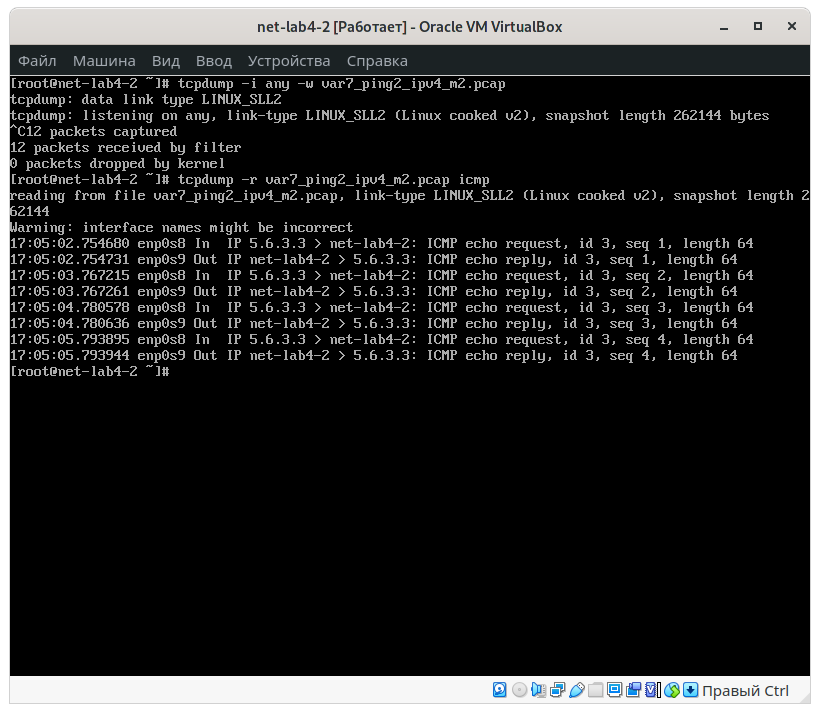
\includegraphics[width=.49\textwidth]{screenshots/var7-ping2-ipv4-tcpdump2}

%    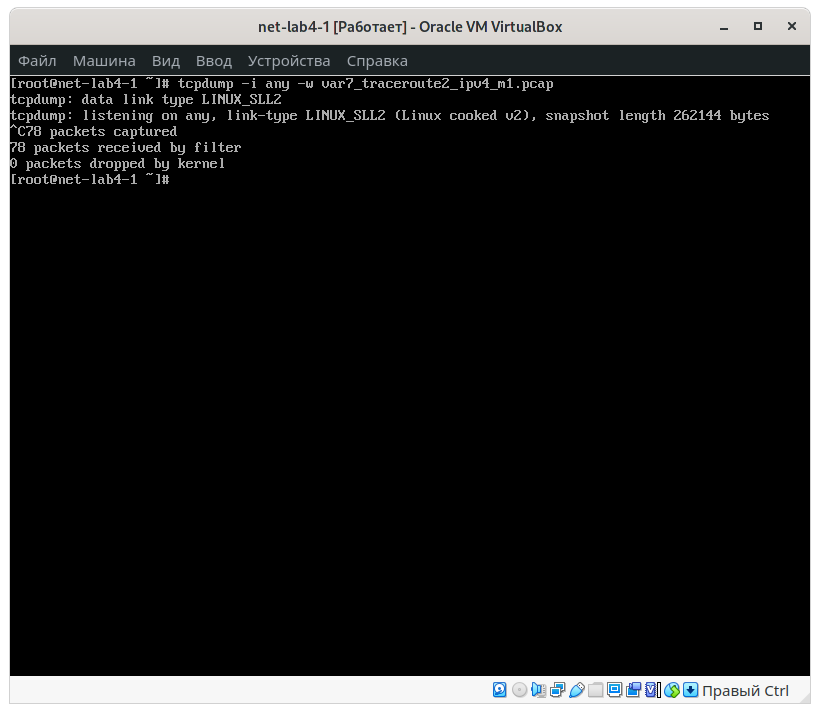
\includegraphics[width=.49\textwidth]{screenshots/var7-traceroute2-ipv4-tcpdump1}
%    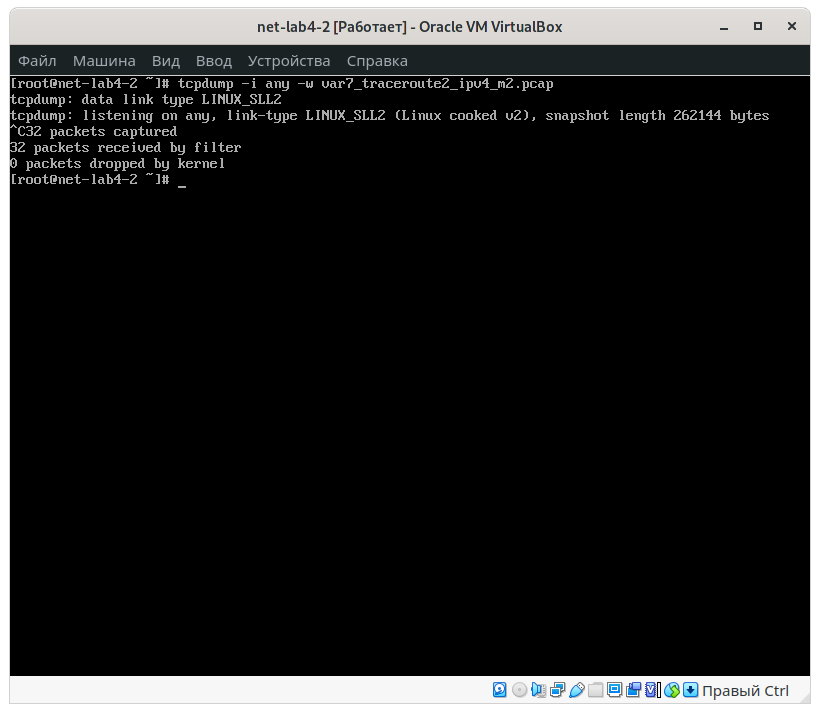
\includegraphics[width=.49\textwidth]{screenshots/var7-traceroute2-ipv4-tcpdump2}
\end{center}

\paragraph{IPv6}
\begin{center}
    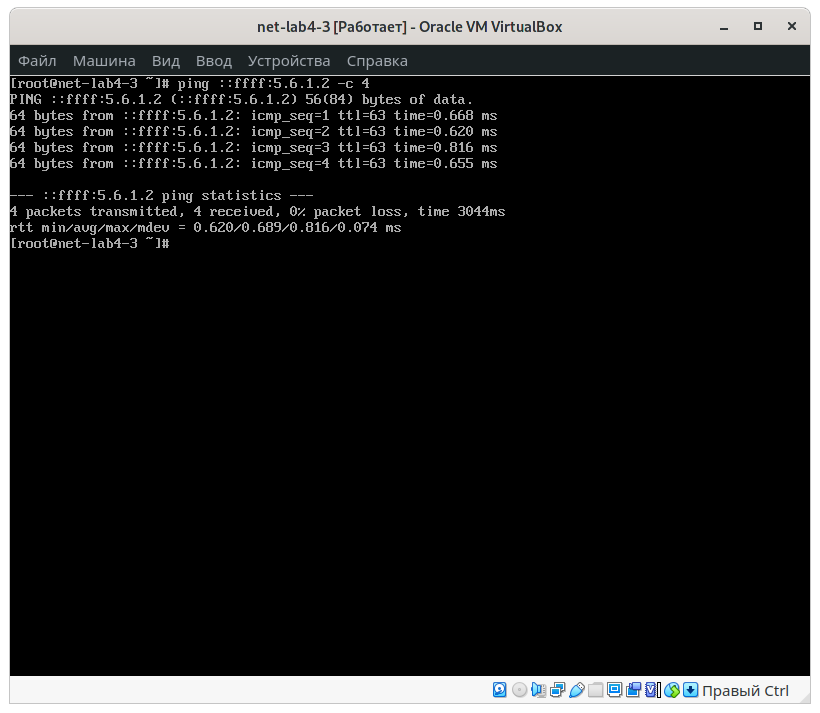
\includegraphics[width=.49\textwidth]{screenshots/var7-ping2-ipv6}
    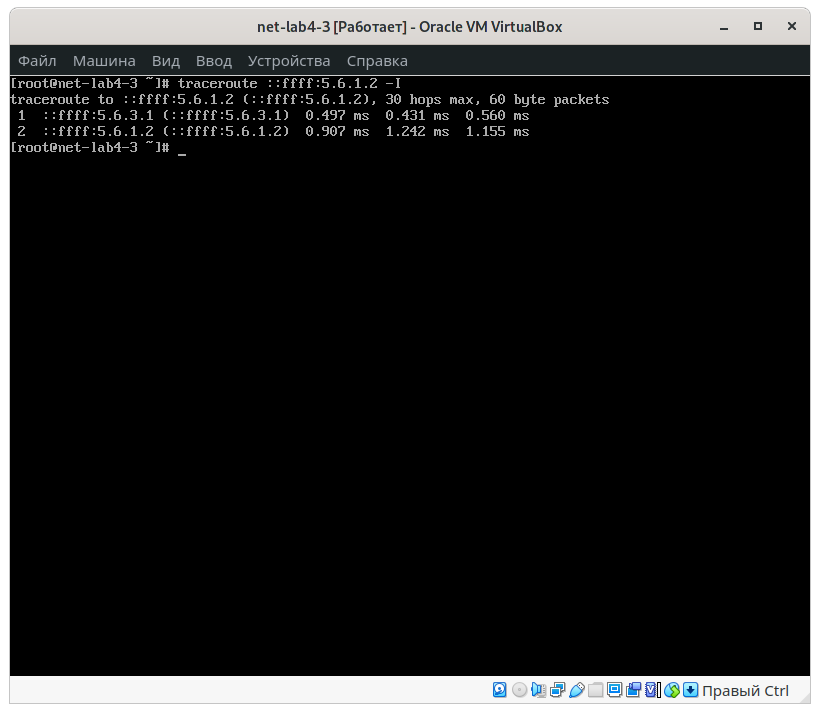
\includegraphics[width=.49\textwidth]{screenshots/var7-traceroute2-ipv6}

    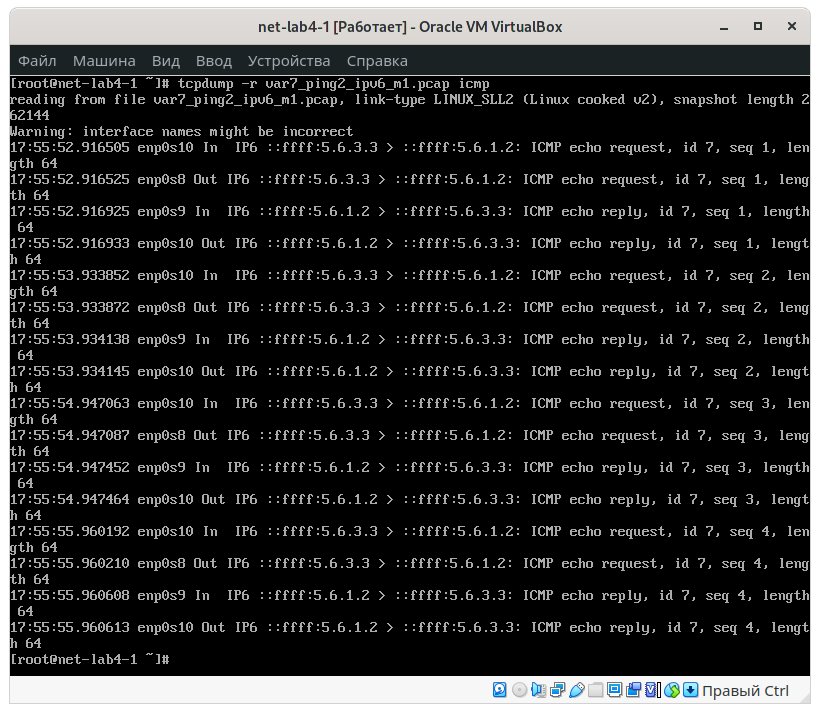
\includegraphics[width=.49\textwidth]{screenshots/var7-ping2-ipv6-tcpdump1}
    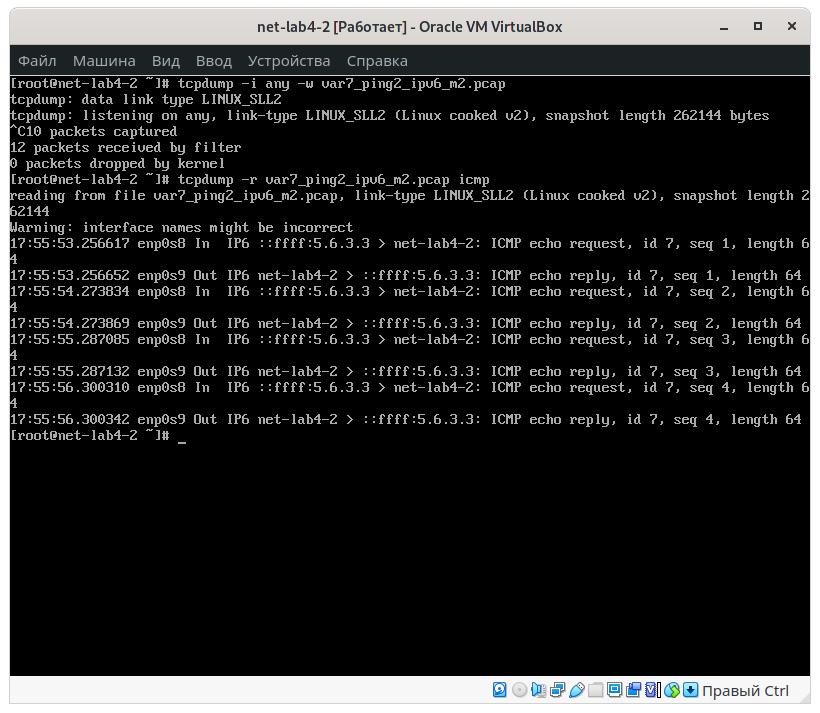
\includegraphics[width=.49\textwidth]{screenshots/var7-ping2-ipv6-tcpdump2}

%    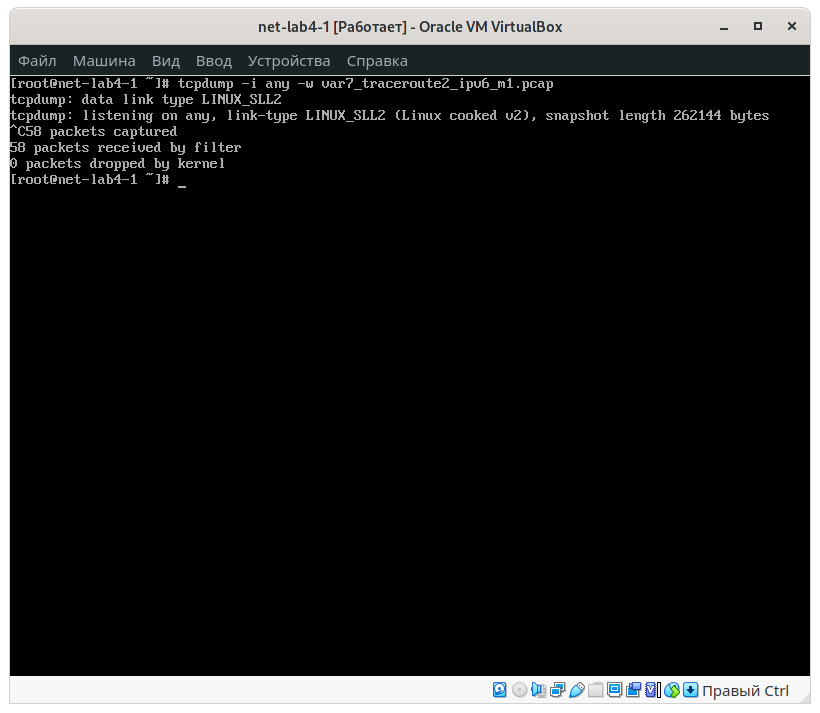
\includegraphics[width=.49\textwidth]{screenshots/var7-traceroute2-ipv6-tcpdump1}
%    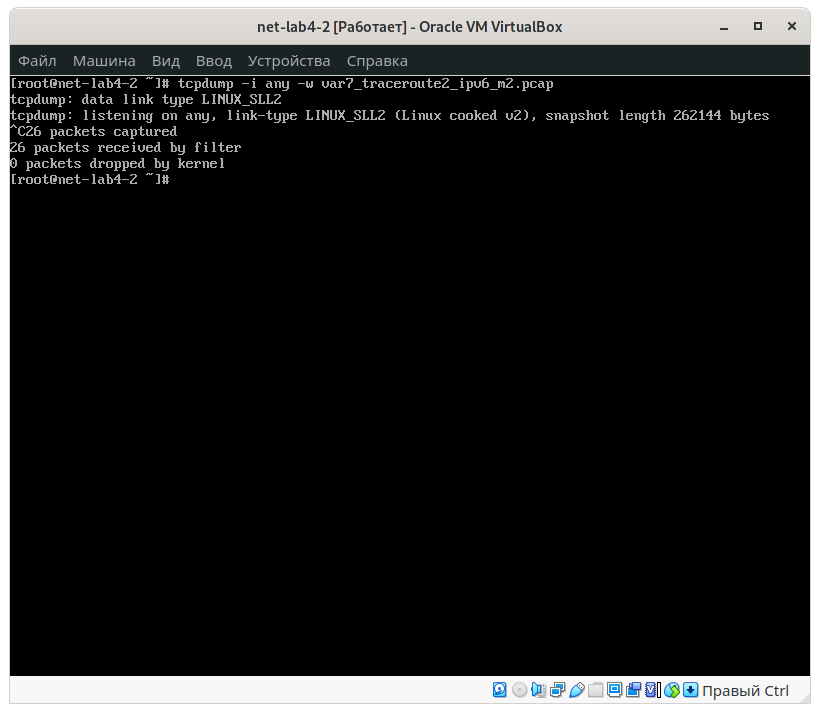
\includegraphics[width=.49\textwidth]{screenshots/var7-traceroute2-ipv6-tcpdump2}
\end{center}
